%!TEX root = ../iotpaper.tex

%~~~~~~~~~~~~~~~~~~~~~~~~~~~~~~~~~~~~~~~~~~~~~~~~~~~~~~~~~~~~~~~


\section{Simultaneous Gestures \\ Experiments}
\label{sec:Simultaneous}
In simultaneous gestures model, we assume the pebble smartwatch as the legitimate prover, an iPhone as the verifier and the other iPhone as the malicious attacker. Three devices starts and ends performing gestures at the same time while the prover and verifier are held together with all axes of accelerometers are correctly corresponded and the attacker is watching and trying to copy the gesture. We tried 4 gestures and each gesture was tested with 10 attempts. The gestures are gesture 5, 7, 11, 17 in \autoref{tab:GestureTable}. Ideally, the prover should be authenticated because it moves together with the legitimate prover and attacker should be denied.

 \begin{figure*}[!t]
% 	\vspace{-1.5em}
    	\centering
 	\subfloat[Gesture \#5 ]{
 	\centering
 	\tikzquarter
		\input{../../Data/plots/simultaneousplots/numeight.tikz}
 		 \label{fig:s5}}
 	\subfloat[Gesture \#7]{
 	\centering
 	\tikzquarter
		\input{../../Data/plots/simultaneousplots/zi.tikz}
 		 \label{fig:s7}}
 	\subfloat[Gesture \#11]{
 	\centering
 	\tikzquarter
		\input{../../Data/plots/simultaneousplots/ru.tikz}
 		 \label{fig:s11}}
	\subfloat[Gesture \#17]{
 	\centering
 	\tikzquarter
		\input{../../Data/plots/simultaneousplots/box.tikz}
 		 \label{fig:s17}}
 	\caption{DTW Distance from both attacker and prover to verifier, separated by gestures, for the Simultaneous Gestures model.}
 	\label{fig:SimultaneousDistanceMatrixPlot}
 \end{figure*}

%\begin{figure}[!tb]
%\centering
%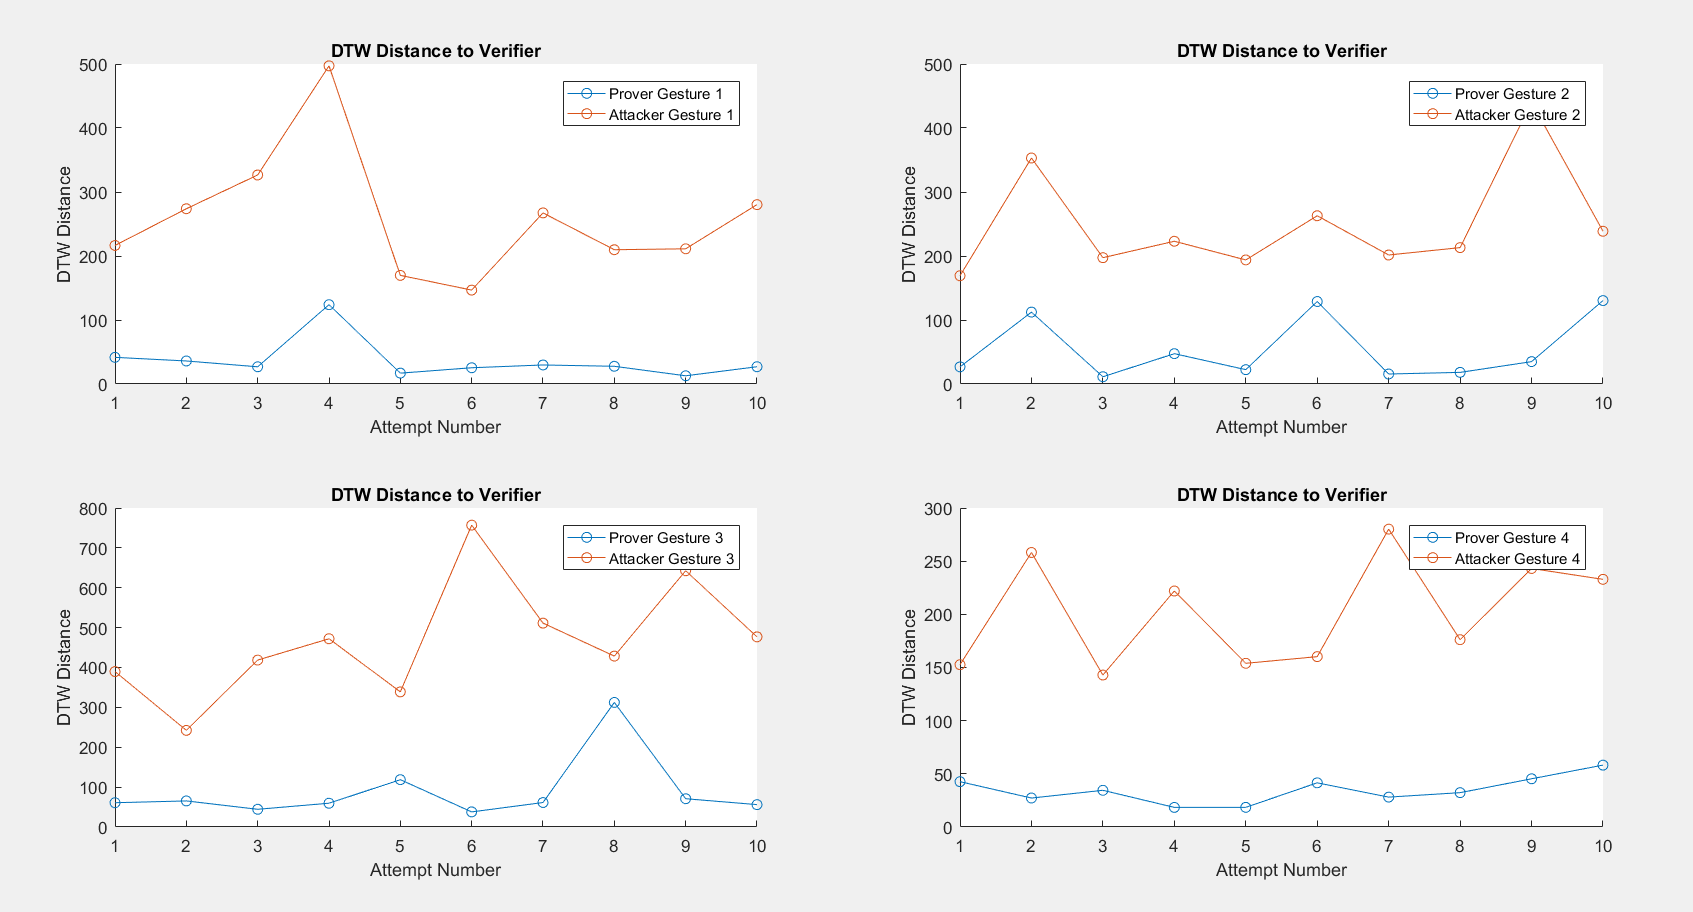
\includegraphics[width= \linewidth]{./figures/simultaneous_model_distance_matrix.png}
%\caption{DTW Distance from both attacker and prover to verifier, separated by gestures.}
%\label{fig:SimultaneousDistanceMatrixPlot}
%\end{figure}

According to the distance matrix we calculated from the raw data, most distance from the prover to the verifier are less than 100 and only 5 samples have distance larger than 100. This shows that when two devices are held together, it is easy to get low distance result between them and this can be exploited for pairing small devices.

The distance between the attacker and the legitimate prover are all larger than 100 and most of them are more then 200. Compared with the distance result of prover, the distance of attacker is always at least 100 larger than that. It is easy to differ the attacker from the prover in  \autoref{fig:SimultaneousDistanceMatrixPlot} so that our simultaneous gestures model works well. 






%~~~~~~~~~~~~~~~~~~~~~~~~~~~~~~~~~~~~~~~~~~~~~~~~~~~~~~~~~~~~~~~
 

